% ─────────────────────────────────────────────────────────────
% src/doc/rho_solver/rho_solver.tex — Approx 引擎 ρ 求解器说明
% 编译（在 src/doc/rho_solver/ 目录下执行）：
%   D:\codeenvset\TinyTeX\bin\windows\xelatex.exe -interaction=nonstopmode rho_solver.tex
% ─────────────────────────────────────────────────────────────
\documentclass[UTF8,10pt]{ctexart}
\usepackage{amsmath,amssymb}
\usepackage{graphicx}
\usepackage{booktabs}
\usepackage[margin=2.2cm]{geometry}
\setlength{\parindent}{2em}
\title{\vspace{-1.2em}ρ 求解器：积分族填充}
\author{}
\date{2026-08}
\begin{document}
\maketitle

\section{ρ 是什么}

Approx 引擎把局面分成两部分：前沿（受数字约束的未知格，按连通块分组，
每个块叫一个组件）和 T 池（无约束的孤立未知格）。全局剩余 $M$ 颗雷
必须在这两部分之间分配。设 $\rho$ 是 T 池的雷密度，守恒方程是
\begin{equation}
F(\rho) = M_{\text{front}}(\rho) + t_{\text{Sum}}\,\rho - M = 0,
\end{equation}
其中 $M_{\text{front}}(\rho)$ 是组件总期望雷数。解出 $\rho$ 之后，
所有格子概率和候选数都由它算出来，所以 $\rho$ 是全局唯一的未知量，
\emph{整个引擎的工作就是把 $M_{\text{front}}(\rho)$ 这个函数定下来}。

组件的精确倾斜期望（指数族公式）是
\begin{equation}
m_i(\rho) = \frac{\sum_k w_k x_k \rho^{x_k - lo_i}(1-\rho)^{hi_i - x_k}}
{\sum_k w_k \rho^{x_k - lo_i}(1-\rho)^{hi_i - x_k}},
\end{equation}
其中 $(w_k, x_k)$ 遍历组件的全部可行方案。这个公式每评估一次就要遍历
一次方案表，所以不能直接用，必须找近似。近似值的好坏由两条性质决定：
\begin{enumerate}
\item \textbf{端点}：$\rho=0$ 时 $m=lo$，$\rho=1$ 时 $m=hi$。
\item \textbf{单调}：$m'(\rho)\ge 0$。不单调的话 $F$ 可能有多个根，
      解不唯一，牛顿法也没有收敛保证。
\end{enumerate}
归一化后写成 $u(\rho)=(M_{\text{front}}-\sum lo)/(\sum hi-\sum lo)$，
$u$ 从 0 走到 1。$p=(\sum mu-\sum lo)/(\sum hi-\sum lo)$ 是组件期望的
归一化位置，$v=\sum\sigma^2/(\sum hi-\sum lo)$ 是归一化方差。

\section{四种填充方案}

四种候选都只用聚合量 $(\sum mu, \sum\sigma^2, \sum lo, \sum hi)$，都是
O(1)。区别在 $u(\rho)$ 取什么形式。

\subsection{无界高斯}
\begin{equation}
u(\rho) = p + \frac{v}{\sum hi - \sum lo}\cdot\ldots \quad
\text{即 } M_{\text{front}} = \sum mu + \sum\sigma^2 \log\tfrac{\rho}{1-\rho}.
\end{equation}
工作原理：$\log\tfrac{\rho}{1-\rho}$ 是 logit 函数，在 $\rho=\frac12$ 处
为零、斜率为 4，向外线性伸展。它在 $\rho=\frac12$ 附近是二阶矩匹配的
好近似，但两端无界——$\rho\to 0$ 时期望趋向 $-\infty$，$\rho\to 1$ 时
趋向 $+\infty$，突破 $[\sum lo, \sum hi]$。实测约 5\% 的局面组件总期望
越界，误差可达 10\% 以上。

\subsection{聚合 clamp}
\begin{equation}
M_{\text{front}}(\rho) = \mathrm{clamp}\!\left(\sum mu + \sum\sigma^2
\log\tfrac{\rho}{1-\rho},\; \sum lo,\; \sum hi\right).
\end{equation}
工作原理：在无界高斯外面套一层钳位，越界部分压回界内。有界性解决了，
但钳位段 $M_{\text{front}}\equiv\sum lo$（或 $\sum hi$），导数恒为 0，
而真实曲线在界内是渐近逼近、导数不为 0。这 0 导数意味着组件对 $\rho$
完全不响应，守恒方程会把"组件真实超出的那点期望"全部塞给 T 池，
$\rho$ 系统性高估。

\subsection{拟合线 $\rho + A\rho(1-\rho)^2$}
\begin{equation}
u(\rho) = \rho + A\,\rho(1-\rho)^2, \qquad
A = -2.853 + 7.2435\,p - 3.1360\,v .
\end{equation}
工作原理：先在真实对局上收集了约 12 万条精确曲线（每局面在 20 个
$\rho$ 采样点用精确倾斜公式算 $M_{\text{front}}$，图~\ref{fig:curve}），
发现聚合曲线近似直线 $u\approx\rho$，带一个中间拱起，拱的形状用
$\rho(1-\rho)^2$ 表示（两端归零、峰在 $\rho=\frac13$）。$A$ 由 $p$、$v$
回归（$R^2=0.9967$）。端点精确、误差很小（平均 0.007--0.06\%），但
$A>3$ 时 $u$ 在 $\rho\approx\frac23$ 处导数变负——基函数表达不了
"位置高且单调"的曲线，0.1\% 的极端局面（$p$ 贴 1、$v$ 极小）会非单调。
要加 cap 缓解。

\subsection{积分族（采用）}
\begin{equation}
u(\rho) = \frac{\int_0^\rho w(t)\,dt}{\int_0^1 w(t)\,dt}, \qquad
w(t) = 1 + k\left(t-\tfrac12\right) + m\left(t-\tfrac12\right)^2 .
\end{equation}
工作原理：先选一个恒正的密度 $w(t)$，再归一化积分。恒正 $\Rightarrow$
$u$ 严格递增；积分自动给出 $u(0)=0$、$u(1)=1$。$w$ 是顶点在
$t=\frac12$ 的二次抛物线，$w(\frac12)=1$ 恒成立，所以恒正条件只需检查
两个端点 $1\pm\frac{k}{2}+\frac{m}{4}>0$。积分结果是归一化三次多项式：
\begin{equation}\label{eq:u}
u(\rho) =
\frac{\rho + \frac{k}{2}\rho(\rho-1)
      + m\left(\frac{\rho^3}{3}-\frac{\rho^2}{2}+\frac{\rho}{4}\right)}
     {1 + \frac{m}{12}} .
\end{equation}
$F'(\rho) = \frac{D\,w(\rho)}{1+m/12} + t_{\text{Sum}} \ge t_{\text{Sum}} > 0$，
单调性是构造出来的，不需要任何补丁。这就是选它的原因。

\section{参数怎么来}

对每条真实曲线解出它的 $(k,m)$（\eqref{eq:u} 对 $k$、$m$ 是线性的，
两边乘 $1+m/12$ 就化成线性最小二乘），然后对全部曲线做回归。数据里
$k$ 与 $p$ 的相关系数是 $-0.98$，$m$ 与 $v$ 是 $-0.99$，所以分开回归：
\begin{equation}\label{eq:km}
k = 3.10326 - 2.46788\,p - 7.16219\,p^2, \qquad
m = 32.7711 - 210.679\,v + 317.91\,v^2 .
\end{equation}
三个约束里有一个是自动的：$\rho=\frac12$ 时 $\log\tfrac{\rho}{1-\rho}=0$，
倾斜权重全部退化为 1，精确公式给出 $u(\frac12)=p$——恒等式，
不依赖拟合。\eqref{eq:km} 预测的 $(k,m)$ 在拟合和样本外数据上
100\% 满足 $1\pm k/2 + m/4 > 0$，即 $w$ 恒正。

\subsection{拟合参数踩过的坑}

积分族不是一步到位的。最早做拟合线方案时，先把 $A$ 当常数直接对
$\rho$ 回归（$A=0.4313$，不依赖任何聚合量），实测根误差 0.12--0.26\%，
比聚合 clamp 还差，不符合预期。排查发现残差 $u-\rho$ 与 $p$
的相关系数是 0.993——几乎完全线性。原因是那条恒等式：
$u(\frac12)=p$ 是精确成立的，而固定 $A$ 的曲线 $u(\frac12)=0.5+\frac18 A$
被钉死在 0.5 附近。真实对局的 $p$ 在 0.50--0.56 之间浮动，固定 $A$
等于给每条曲线配一个错误的中点，根误差就是锚点偏移传导到 $\rho$ 的结果。

于是把 $A$ 改成 $p$、$v$ 的回归：$A=-2.853+7.2435p-3.1360v$，
$R^2=0.9967$，误差立刻跌到 0.007--0.067\%，降了一个数量级。
再换积分族时延续同样的结构。这个教训是：\textbf{$mu$ 和 $\sigma^2$
不是可选的附加特征——$mu$ 是曲线的锚点（经恒等式直接钉死中点），
$\sigma^2$ 是曲线的陡峭度，它们承载了曲线最核心的信息，
不喂给回归就会系统性偏差}。

\section{求解流程}

\texttt{Approx::solveRho} 的实际流程：
\begin{enumerate}
\item $M\le\sum lo$：$\rho=0$（雷数连组件下限都填不满，T 池零雷）；
      $M\ge\sum hi+t_{\text{Sum}}$：$\rho=1$。这些量全是整数，
      判定是精确的。
\item $D=\sum hi-\sum lo=0$（组件全确定性）：$u$ 无定义，退化为线性
      解析解 $\rho=(M-\sum mu)/t_{\text{Sum}}$。
\item 一般情形：算 $p$、$v$，代入 \eqref{eq:km} 得 $k$、$m$，对单调
      三次方程做带界牛顿。初值取线性填充解
      $\rho_0=(M-\sum lo)/(D+t_{\text{Sum}})$，实测 1--2 次收敛。
\end{enumerate}
聚合量由观察者模式 O(1) 增量维护，求解全程不枚举任何组件。

\section{误差数据}

图~\ref{fig:curve} 是五盘面实测曲线的样子（基本贴对角线，中间略拱），
图~\ref{fig:resid} 是残差。表~\ref{tab:err} 是各方案解出的 $\rho$ 与
精确根（300 次二分精确曲线）的差距，样本外种子。

\begin{figure}[htbp]\centering
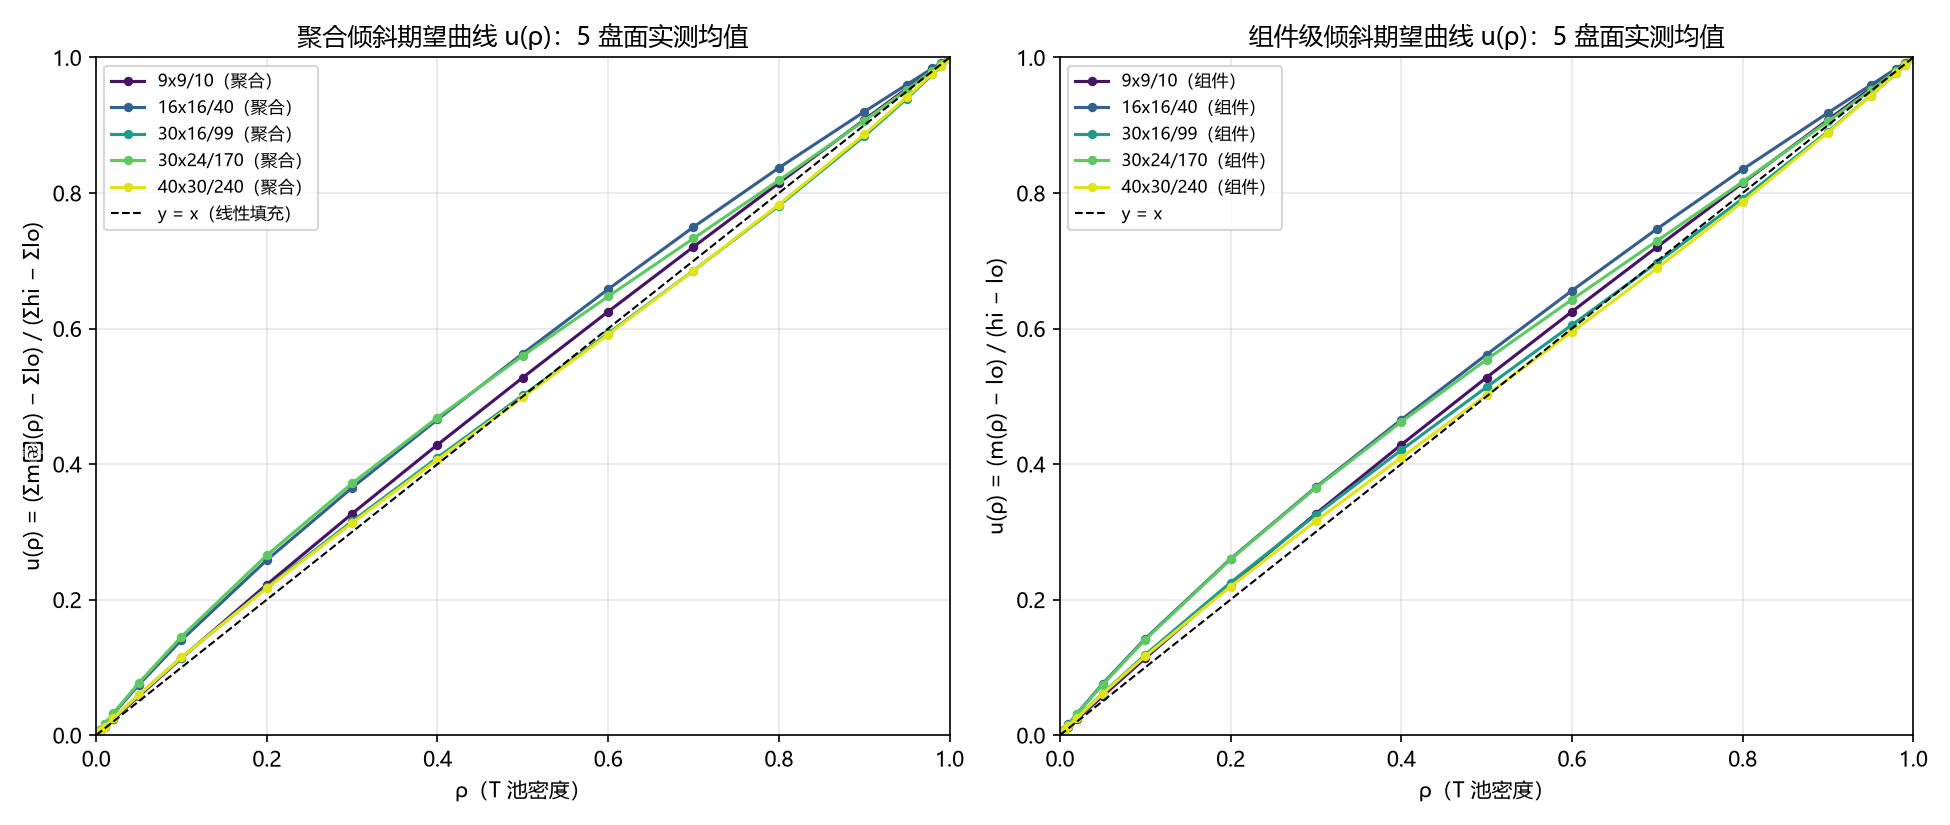
\includegraphics[width=0.75\linewidth]{u_curve.png}
\caption{五盘面聚合曲线 $u(\rho)$ 实测均值，黑虚线是 $u=\rho$。}
\label{fig:curve}
\end{figure}

\begin{figure}[htbp]\centering
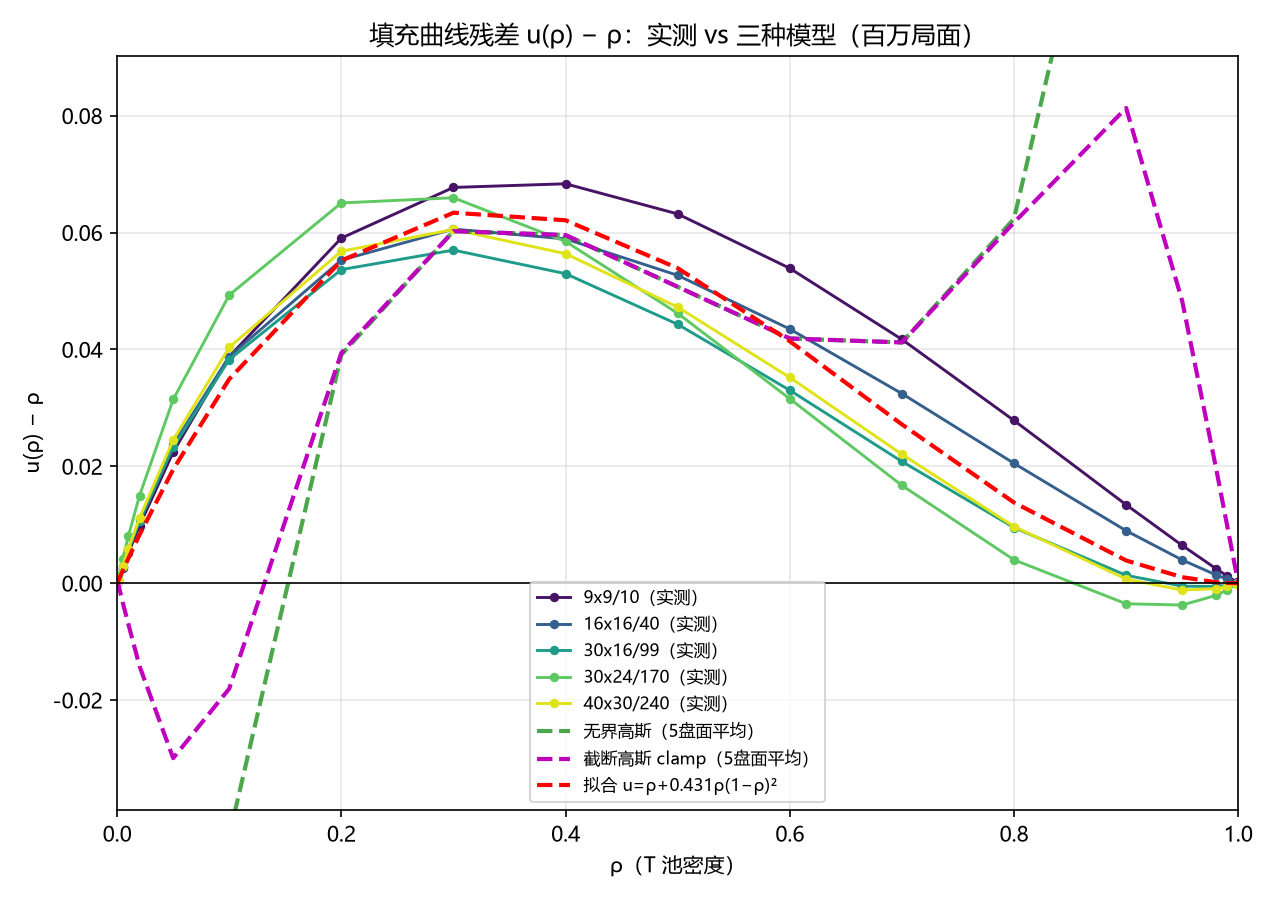
\includegraphics[width=0.75\linewidth]{resid_curve.png}
\caption{残差 $u(\rho)-\rho$。绿线（无界高斯）两端爆炸，没参与纵轴标定。}
\label{fig:resid}
\end{figure}

\begin{table}[htbp]\centering
\caption{根误差（\%），样本外。}
\begin{tabular}{lcccc}
\toprule
方案 & 平均 & 最大 & $>1\%$ 计数 & 单调性 \\
\midrule
无界高斯 & 0.064--0.97 & 11.8 & 多 & 无界，不适用 \\
聚合 clamp & 0.012--0.30 & 2.8 & 少数 & 硬切，导数归零 \\
拟合线（cap） & 0.014--0.059 & 1.1 & 1--5 & 靠 cap 缓解 \\
积分族 & 0.0068 & 0.139 & 0 & 构造保证 \\
\bottomrule
\end{tabular}
\end{table}

回归测试：observe\_brute\_test 16619 项、observe\_exact\_test
30844 项，全部通过。

\end{document}